\documentclass[10pt,a4paper]{paper}
\usepackage[utf8]{inputenc}
\usepackage{amsmath}
\usepackage{amsfonts}
\usepackage{amssymb}
\usepackage{graphicx}
\graphicspath{ {./} }
\author{Aaron Winziers und Michael Wolz}
\title{2. Übung Rechnernetze}
\begin{document}
	
	\maketitle
	
	\section*{Aufgabe 2}
	
	Zuerst haben wir mittels der Literatur die Worst-Case Laufzeit des Programms berechnet. Dazu haben wir folgende Formeln verwendet:
	\begin{itemize}
		\item Laufzeit von Breadth-First Search: $O(E+V)$
		\item Anzahl der von uns verwendeten Kanten: $V-1$
		\item Anzahl der Knotenpaare: $\frac{V(V-1)}{2}$
	\end{itemize}

	Durch einsetzen der Kantenzahl in der Laufzeit des Algorithmus und anschließende Multiplikation mit der Anzahl der benötigten Durchläufe haben wir folgende Formel erzeugt:
	\begin{center}
		$O(\frac{2V^{3}-3V^{2}+V}{2})$
	\end{center}
	
	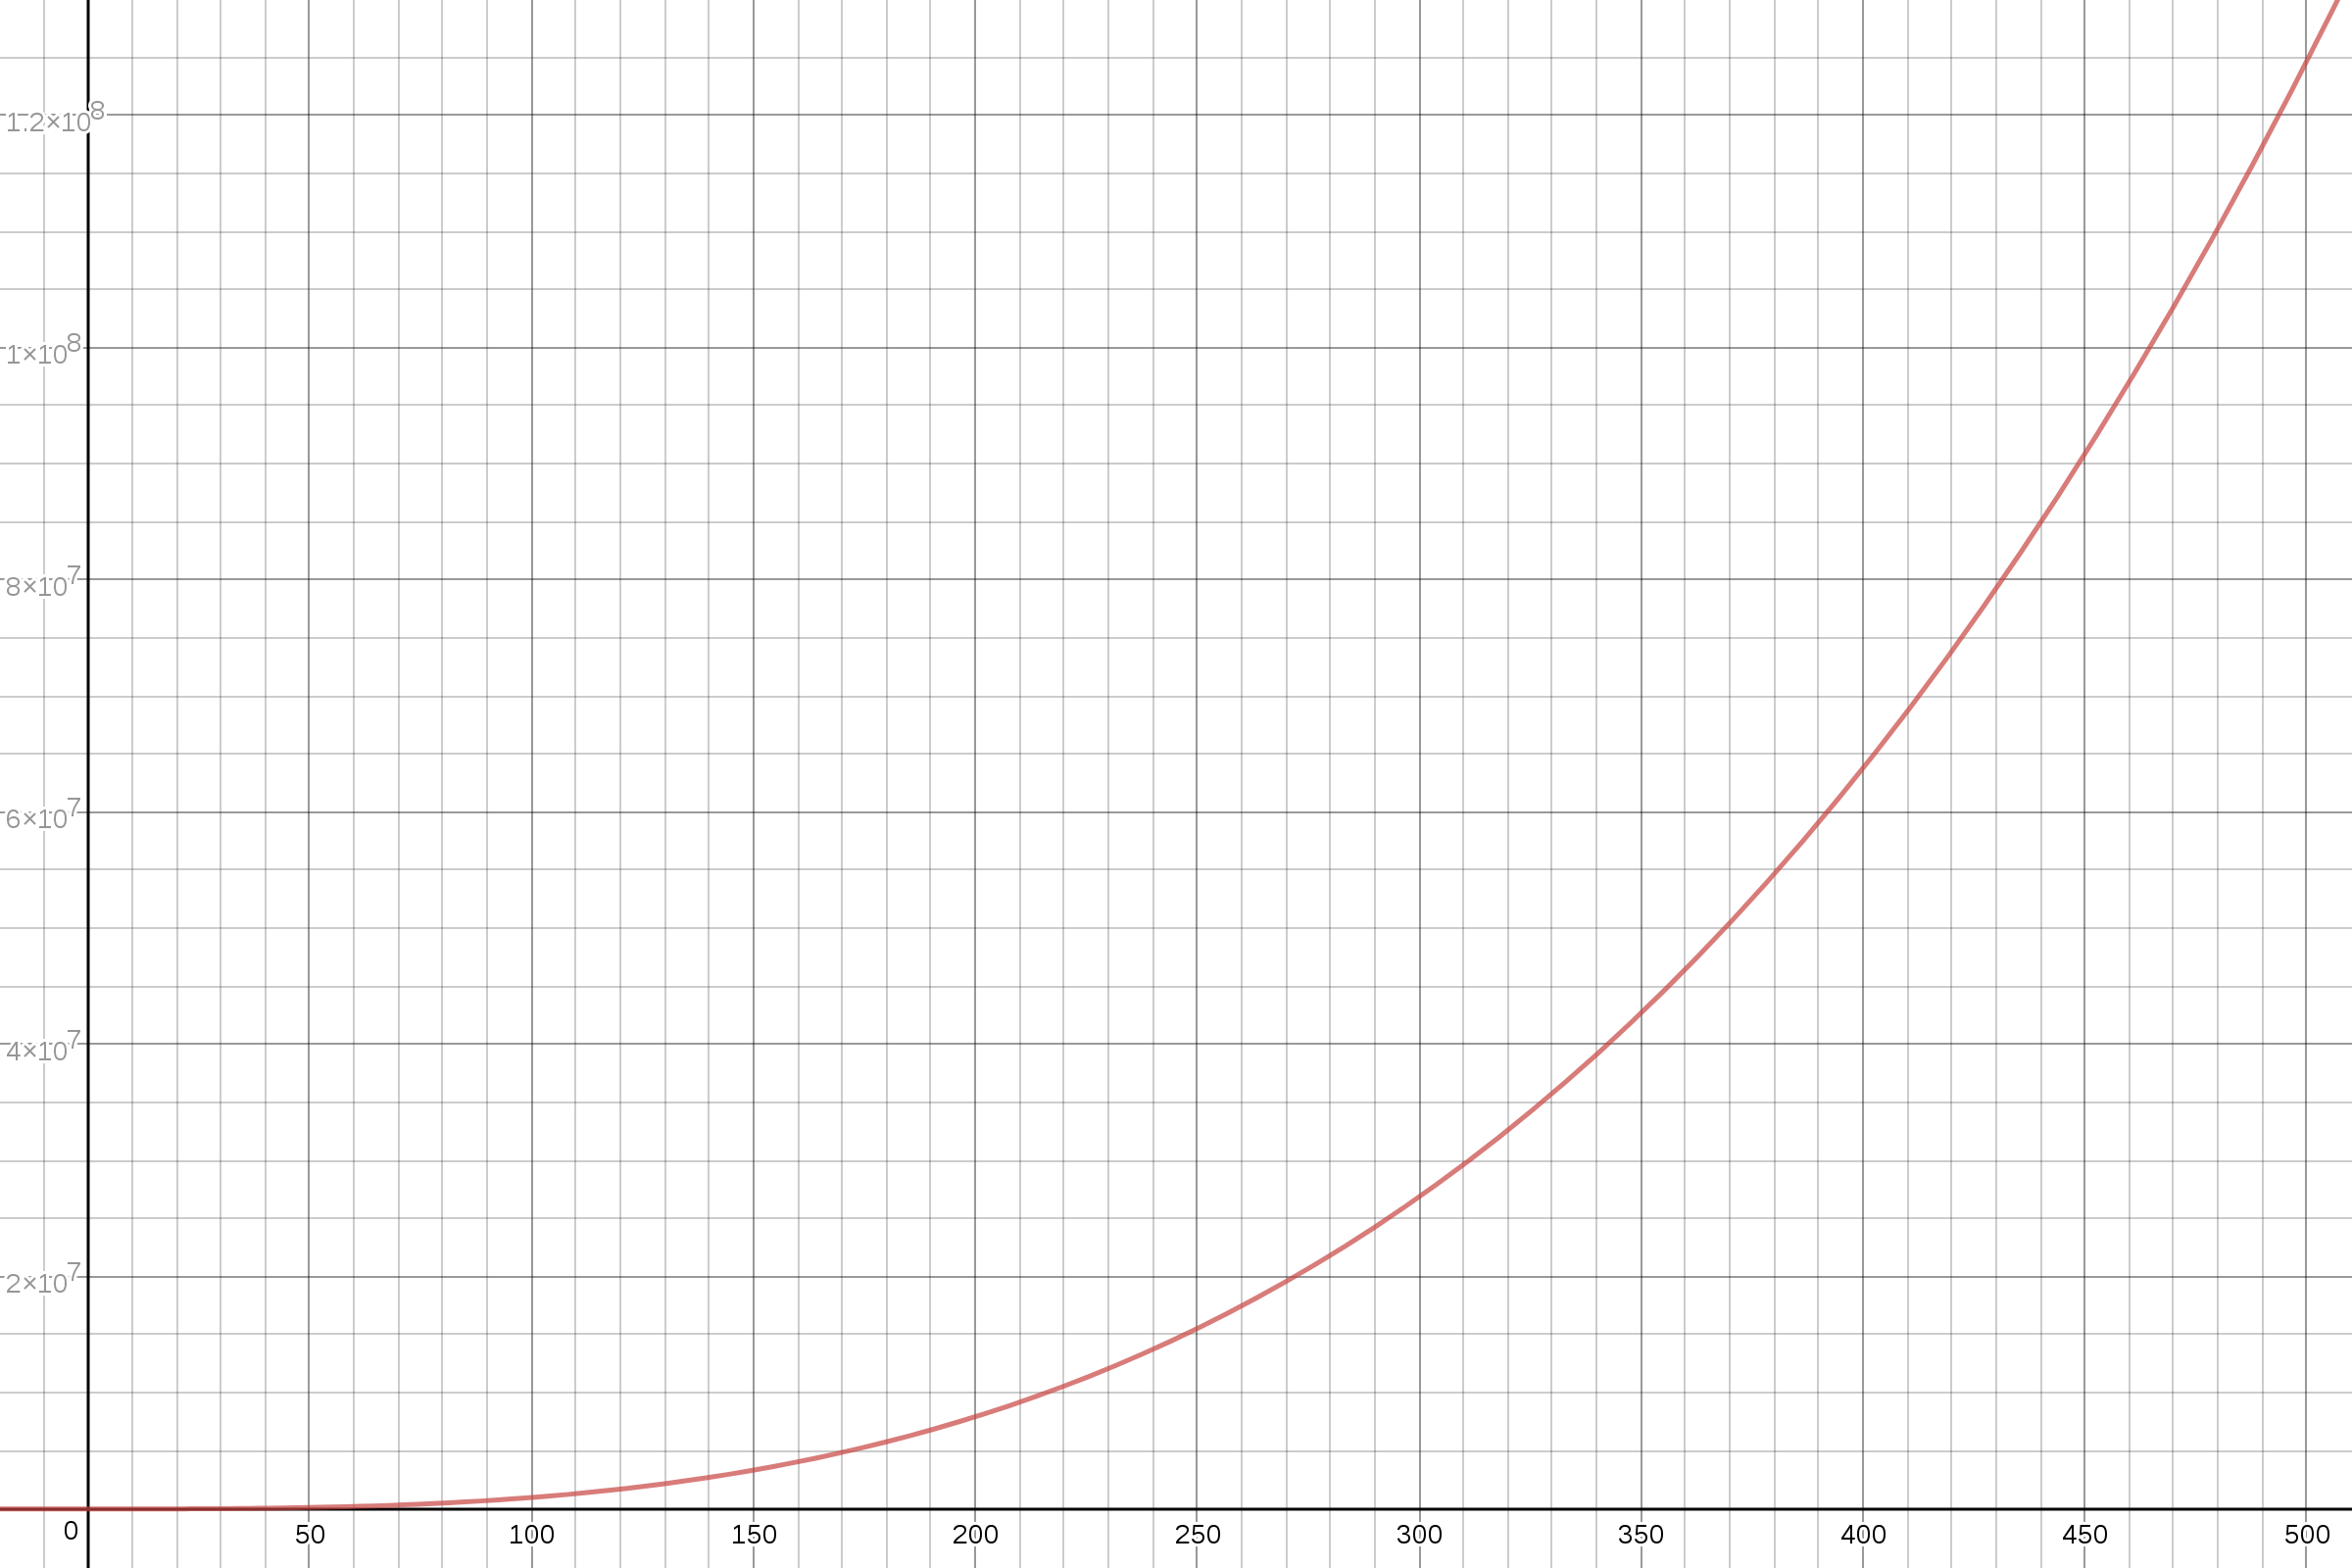
\includegraphics[width=0.5\textwidth]{desmos-graph.png}
	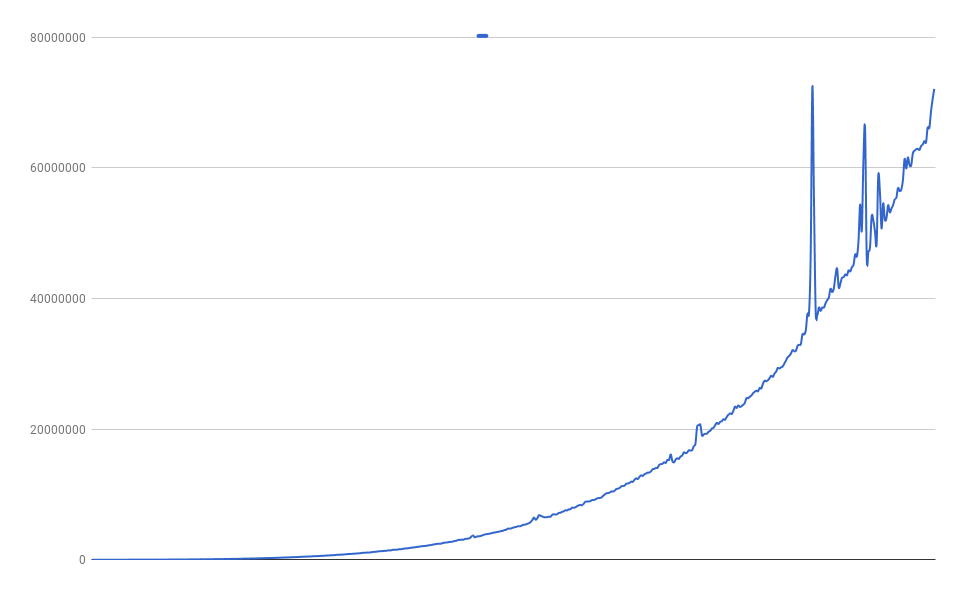
\includegraphics[width=0.5\textwidth]{chart.png}
	
	In den obigen Graphen ist Links die von uns geschriebene Funktion und Rechts die Daten die wir durch das Programm gesammelt haben. Die Abbildungen lassen sich gut vergleichen und die Daten bestätigen das was in der Literatur steht.
	
	\par 
	
	Sollte man das Programm über das Internet laufen lassen würde es extreme Zeit in Anspruch nehmen um alle Berechnungen fertig zu machen. Bei einem Durchlauf mit 100.000 Knoten haben wir das Programm nach ca. 5 Minuten abgebrochen, also würde das Programm vermutlich bei 8+ Mrd. Knoten Mehrere Stunden wenn nicht Tage brauche um Erfolgreich zu terminieren.
	
\end{document}